\documentclass[11pt, spanish]{article}
\usepackage{amssymb, amscd, amsthm, amsfonts, mathtools, mathrsfs, tensor, braket, etoolbox}
\numberwithin{equation}{section}
\mathtoolsset{showonlyrefs,showmanualtags}
\usepackage{graphicx, float}
\usepackage{asymptote}

\usepackage{hyperref}
\hypersetup{
colorlinks=true,
urlcolor = cyan,
linkcolor=blue,
citecolor=brown}
\usepackage[spanish,es-nodecimaldot, es-tabla]{babel}
\usepackage{siunitx}
\sisetup{separate-uncertainty}
\DeclareSIUnit{\atm}{\text{atm}}

\usepackage{upgreek}
\usepackage[minimal = true]{chemmacros}
\usepackage{cancel}

\usepackage{multicol, multirow}
\usepackage{wrapfig}

%\usepackage{blindtext}

\usepackage[lastexercise]{exercise}
\renewcommand{\AtBeginExercise}{\itshape}

\usepackage{booktabs}

\setlength{\headheight}{14pt}

\usepackage{lastpage}

\usepackage[margin=2.5cm]{geometry}

\usepackage{esint}
\usepackage{booktabs}


\usepackage{enumerate}
\usepackage{nicefrac}


\usepackage[font=small]{caption}
\usepackage{subcaption}

\usepackage{esint, csquotes}
\usepackage[
	backend=biber,
	style=apa
]{biblatex}
\addbibresource{Bibliografia.bib}
\usepackage{xurl}

% \usepackage[skip=10pt plus80pt]{parskip}

\setlength{\headheight}{14pt}

\oddsidemargin 0pt
\evensidemargin 0pt
\marginparwidth 40pt
\marginparsep 10pt
\topmargin -20pt
\headsep 10pt
\textheight 8.7in

\renewcommand{\vec}{\mathbf} %Reescribe a los vectores en negritas y no con una flechita
\newcommand{\univ}[1]{\, \hat{\vec{#1}}} % Facilita la escritura de vectores unitarios
\newcommand{\eqcomma}{\,  ,}
\newcommand{\R}{\mathbb R}
\newcommand{\C}{\mathbb C}
\renewcommand{\r}{\vec r}
\newcommand{\eqperiod}{\,  .}
\newcommand{\bfgreek}[1]{\boldsymbol{#1}}
\newcommand{\surface}{\mathcal S}
\newcommand{\tangent}{\boldsymbol{\mathfrak{t}}}
\newcommand{\normal}{\boldsymbol{\mathfrak{n}}}
\newcommand{\binormal}{\boldsymbol{\mathfrak{b}}}
\newcommand{\bracket}[1]{\left\langle #1 \right\rangle}
\newcommand{\jacobian}[2]{\frac{\partial(#1)}{\partial(#2)}}
\newcommand{\EC}[1][1]{\frac{#1}{4\pi\epsilon_0}}
\newcommand{\dotp}[2]{\vec{#1} \cdot \vec{#2}}
\newcommand{\crossp}[2]{\vec{#1} \times \vec{#2}}
\newcommand{\Matrix}[1]{\begin{pmatrix}#1\end{pmatrix}} 

\renewcommand\qedsymbol{$\blacksquare$}%Hace un cuadrado negro el qed de una demostración
\newtheorem{theorem}{Teorema} %Crea el entorno de teorema
\newtheorem{corollary}{Corolario}
\newtheorem{lemma}{Lema}
\newtheorem{definition}{Definición}

\newcommand{\eto}[1]{e^{#1}}
\renewcommand{\div}[1]{\nabla \cdot \vec{#1}}
\newcommand{\rot}[1]{\nabla \times \vec{#1}}

\DeclareMathOperator{\arccot}{arccot}
\DeclareMathOperator{\arcsenh}{arc\ senh}
\DeclareMathOperator{\Span}{span}

\DeclarePairedDelimiter{\abs}{\lvert }{\rvert}
\DeclarePairedDelimiterX{\norm}[1]{\lVert}{\rVert}{\ifblank{#1}{\:\cdot\:}{#1}}
\DeclarePairedDelimiterXPP{\lnorm}[2]{}{\lVert}{\rVert}{_\ifblank{#2}{2}{#2}}{\ifblank{#1}{\: \cdot \:}{#1}}
\DeclarePairedDelimiterX{\innerp}[2]{\langle}{\rangle}{#1 \delimsize \vert \mathopen{} #2}
\DeclarePairedDelimiterX{\scalarp}[2]{\langle}{\rangle}{#1 , #2}


\usepackage{titlesec}

\titleformat*{\section}{\large\bfseries}
\titleformat*{\subsection}{\large\bfseries}
\titleformat*{\subsubsection}{\large\bfseries}
\titleformat*{\paragraph}{\large\bfseries}
\titleformat*{\subparagraph}{\large\bfseries}

\title{
	\textbf{Práctica 8\\
	Polarización de la Luz}
}
\author{Luis Arturo Ureña Casarrubias\\
Laboratorio de Óptica}
\date{\today}


\begin{document}

\maketitle

\abstract{
	La polarización de la luz es una propiedad fundamental de la luz como onda electromágnética y que el ser humano le ha encontrado diversos usos a lo largo de la historia. Nuestro objetivo fue obtener una ley de la intensidad medida de un láser rojo de \qty{632}{\nm}, linealmente polarizado, al pasar por un polarizador, partiendo de las ecuaciones de Maxwell y empleando el cálculo matricial de Jones.
}

\begin{multicols}{2}

\section{Introducción}
%La difracción, como consecuencia de la naturaleza ondulatoria de la luz, está más difundida en el imaginario colectivo a través del experimento de la doble rendija de Young y su relación con la mecánica cuántica.

Es más probable, sin embargo, que la difracción de la luz pase completamente desapercibida en la vida diaria, o cuando menos, no es nombrada como tal.  Este fenómeno se presenta en las sombras difuminadas que proyecta un objeto sobre una superficie cuando hay una distancia considerable entre ellos, como se muestra en la figura~\ref{fig: blurry}. 

\begin{figure}[H]
	\centering
	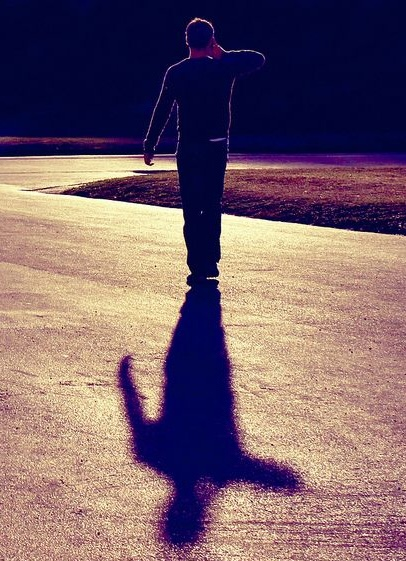
\includegraphics[width=.4\linewidth]{Imagenes/blurry_shadow}
	\caption{La sombra proyectada se difumina conforme el punto de proyección en el suelo se aleja del hombre que bloquea la luz. Imagen recuperada de \parencite{blurry_shadow}.}
	\label{fig: blurry}
\end{figure}

El primer informe del cual se tiene registro sobre la difracción de la luz es el trabajo del sacerdote jesuita y físico-matemático Francesco Maria Grimaldi \textit{Physico-mathesis de lumine, coloribus et iride aliisque adnexis} de 1665 \parencite{Grimaldi}, obra donde acuñó el término \emph{difracción} y que fue posteriormente citado por personajes como Newton y Huygens.

La polémica entre las teorías corpusculares y ondulatorias sobre la luz de Newton y Huygens, respectivamente, es bien conocida. Menos conocidos son los conceptos ondulatorios en la óptica de Newton.  En 1675 formuló una hipótesis consistente de seis puntos donde enumeraba algunas de las propiedades que debía poseer el éter, mas no identificaba a las vibraciones de este medio con la luz, sino que estos dos influían mutuamente entre sí: el primero refractaba al segundo y el segundo lo ``calentaba'' \parencite{stuewer-1970}.

Otro físico contemporáneo y de renombre que apoyaba la teoría ondulatoria de la luz fue Robert Hooke, y a cuyos argumentos Newton respondía en parte con aprobación, ya que podría explicar entonces la sensación de color en el ojo como la recepción de ondas luminosas así como el oído capta ondas sonoras, en parte con desaprobación, pues la propagación de la luz como una onda no explicaría como podría ser entonces en línea recta y entonces no se podrían formar sombras.

Newton entonces propusó en 1675 que la difracción de la luz en el doblamiento hacia la sombra geométrica de un objeto era una forma de refracción continua provocada por un gradiente en el éter que rodeaba a los objetos.  Sin embargo, hay evidencia para demostrar que no hasta después de 1678 que él mismo realizó experimentos sobre la difracción de la luz.

Un siglo después, en 1801, el físico inglés Thomas Young obtuvó nueva evidencia a favor del modelo ondulatorio de la luz en una época donde la teoría de Newton ya había sido ampliamente aceptada. Young reflejó con un espejo luz solar sobre un agujerito para que atravesará horizontalmente un cuarto oscuro \parencite{Young-1804}.  Después dividió este rayo con un pedazo de papel con un grosor de \qty{.195}{\cm} y observó la sombra proyectada, donde distinguió bandas de colores a cada lado de la sombra, pero más importante, bandas brillantes y oscuras, como se muestran en la figura~\ref{fig: double_slit}.

\begin{figure}[H]
	\centering
	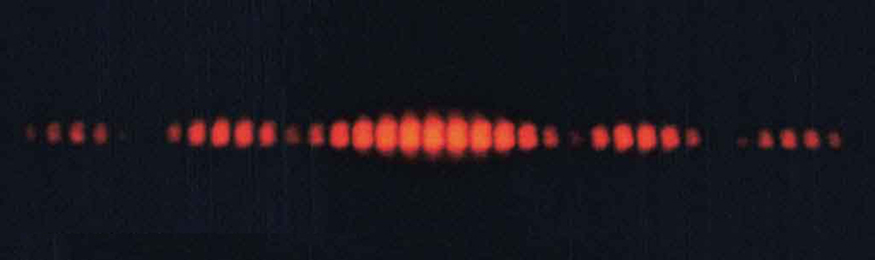
\includegraphics[width=.7\linewidth]{Imagenes/diffraction}
	\caption{Patrón de difracción similar al que debió observar Thomas Young en su experimento de 1801. Imagen recuperada de \parencite{openstax}.}
	\label{fig: double_slit}
\end{figure}

%\section{Polarización: una descripción matemática}\label{sec: teo}

Para estudiar la propagación de la luz como una onda electromagnética consideramos el caso especial de las ecuaciones de Maxwell en el vacío y sin fuentes.
\begin{align}
    \div E &= 0, & \rot E + \partial_t \vec B &= 0\\
    \div B &= 0, & \rot B - \frac{1}{c^2}\partial_t \vec E &= 0.
\end{align}

Al desacoplarlas obtenemos que los campos $\vec E$ y $\vec B$ satisfacen ecuaciones de onda
\begin{equation}
    \nabla^2 \vec E = \frac{1}{c^2}\partial^2_t \vec E, \qquad \nabla^2 \vec B = \frac{1}{c^2}\partial^2_t \vec B.
\end{equation}

Lejos de las fuentes, podemos aproximar a estas ondas como ondas planas con frecuencia angular $\omega$ que se propagan en la dirección $\vec k$.
\begin{gather}
    \vec E(\r, t) = \vec E_0 \cos(\dotp k r - \omega t),\\
    \vec B(\r, t) = \vec B_0 \cos(\dotp k r - \omega t),
\end{gather}
donde $\norm E = c\norm B$.

Para estudiar la polarización de la luz, como esta está definida en términos del campo eléctrico, reescribimos la ecuación de onda para el campo eléctrico en notación compleja
\begin{equation}
    \tilde{\vec E}(\r, t) = \tilde{\vec E}_0 \eto{i(\dotp k r - \omega t)},
\end{equation}
donde $\tilde{\vec E}_0$ es un vector complejo. En esta ecuación el campo eléctrico físico se obtiene tomando la parte real de $\tilde{\vec E}$.

Si tomamos al eje $z$ como la dirección de propagación de la onda, entonces podemos escribir
\begin{equation}\label{eq: complexE}
    \tilde{\vec E} = \eto{i(kz - \omega t)}(\tilde{E}_{0x}  \vec i + \tilde{E}_{0y}  \vec j),
\end{equation}
y al expresar a las componentes en forma polar
\begin{equation}\label{eq: amplitudes}
    \tilde{E}_{0x} = E_{0x}\eto{i\phi_x},
    \tilde{E}_{0y} = E_{0y}\eto{i\phi_y},
\end{equation}
podemos obtener los distintos tipos de polarización. Si $\phi_x = \phi_y = \phi$, entonces
\begin{gather}
    \tilde{\vec E} = \eto{i(kz - \omega t + \phi)}(E_{0x}  \vec i + E_{0y}  \vec j),\\
    \vec E = \cos(kz - \omega t + \phi)(E_{0x}  \vec i + E_{0y}  \vec j),
\end{gather}
es decir, $\vec E$ oscila en una sola dirección y decimos entonces que está \emph{linealmente polarizada}.

Si $\phi_y = \phi_x - \pi/2$,
\begin{equation}\label{eq: elliptical}
    \tilde{\vec E} = \eto{i(kz - \omega t + \phi_x)}(E_{0x}  \vec i - i E_{0y}  \vec j),
\end{equation}
\begin{multline}
    \vec E = E_{0x}\cos(kz - \omega t + \phi_x)\vec i\\
    + E_{0y}\sen(kz - \omega t + \phi_x)\vec j,
\end{multline}
y el campo eléctrico rota en sentido antihorario sobre una elipse y decimos que tiene una \emph{polarización elíptica izquierda}; la polarización elíptica derecha se obtiene cuando $\phi_y = \phi_x + \pi/2$, y si a la vez $E_{0x} = E_{0y} = E_0$,
\begin{equation}
    \vec E = E_0(\cos(kz - \omega t + \phi_x) \vec i + \sen(kz - \omega t + \phi_x)  \vec j),
\end{equation}
y en este caso el campo eléctrico rota sobre una circunferencia y decimos que tiene una polarización \emph{circular}.

Experimentalmente no se mide como varía el campo eléctrico, pues para el espectro visible las frecuencias $\omega$ son del orden de \qty{1e15}{\Hz}. Entonces, al hacer una medición lo que se está midiendo es el promedio de la potencia por unidad de área que transmite la onda, o \emph{irradiancia} $I$ que se calcula como
\begin{equation}
    I = \braket{S},
\end{equation}
donde $S$ es la magnitud del vector de Poynting
\begin{equation}
    \vec S \coloneq \frac{1}{\mu_0} \crossp{E}{B}.
\end{equation}
Para ondas monocromáticas, como las del láser rojo que empleamos,
\begin{equation}
    \vec S = \frac{1}{c\mu_0} E^2 \vec k = c\epsilon_0 E_0^2 \cos^2(kz - \omega t + \phi) \vec k.
\end{equation}
Entonces
\begin{equation}\label{eq: irradiance}
    I = \frac12 c\epsilon_0 E_0^2.
\end{equation}

\subsection{Ley de Malus}

En la primera parte de la práctica introducimos un polarizador lineal entre la fuente, el láser rojo, y el medidor de potencia. Un polarizador lineal es un elemento óptico que, a través de diversos mecanismos como sería el \emph{dicroísmo}, la reflexión, la dispersión o la doble reflexión, separa las polarizaciones de la onda eléctrica y transmite solamente una de ellas \parencite{hecht-1999}. Esta separación se observa en que existe una dirección preferencial del polarizador que permite la máxima transmisión de luz polarizada lineal incidente en él; esta dirección se denomina \emph{eje de transmisión} \parencite{fowles-1989}. Un polarizador ideal es uno que transmite totalmente a luz polarizada paralelamente a su eje de transmisión y que absorbe totalmente luz polarizada perpendicularmente a su eje.

Este eje de transmisión define el subespacio unidimensional $U = \Span \univ n$, donde $\univ n$ es un vector unitario paralelo al eje de transmisión del polarizador lineal. Podemos entonces separar al espacio $\R^3$ como la suma directa $\R^3 = U\oplus U^{\perp}$, es decir, existen vectores únicos y ortogonales entre sí $\vec E_1 \in U$ y $\vec E_2 \in U^{\perp}$ tales que
\begin{equation}
    \vec E_0 = \vec E_1 + \vec E_2.
\end{equation}
El vector $\vec E_1$ se obtiene como
\begin{equation}\label{eq: proj}
    \vec E_1 = (\dotp{\vec E}{\univ n})\univ n = E\cos\phi \univ n,
\end{equation}
donde $\phi$ es el ángulo que forma $\vec E_0$ con $\univ n$. Este es el campo eléctrico que será detectado después de que haya atravesado al polarizador lineal. Sustituyendo en la ecuación \eqref{eq: irradiance}
\begin{equation}
    I(\phi) = \frac12 c\epsilon_0 (E_0\cos\phi)^2 = \frac12 c\epsilon_0 E_0^2 \cos^2\phi.
\end{equation}
Si definimos $I_0 = c\epsilon_0 E_0^2/2$, entonces obtenemos la \emph{Ley de Malus}
\begin{equation}\label{eq: Malus}
    I(\theta) = I_0 \cos^2\phi.
\end{equation}
Con esta ecuación podemos determinar, hasta un múltiplo entero de $\pi$, el eje de transmisión de un polarizador lineal, siempre y cuando la luz incidente esté polarizada linealmente.

Si la luz incidente no está polarizada linealmente, o tiene una polarización circular, entonces todos los valores de $\phi$ ocurren con igual probabilidad y lo que se mide es el promedio sobre todos los ángulos. Como $\braket{\cos^2 \phi} = 1/2$, entonces la ley de Malus es
\begin{equation}
     I(\phi) = \frac{I_0}{2}.
\end{equation}

\subsection{Cálculo de Jones: Álgebra Lineal en la Óptica}

Tomando nuevamente una onda electromagnética que se propaga en la dirección $z$, y usando la descripción compleja, es apropiado entonces usar el espacio vectorial $\C^2$ con su base canónica y el producto interno Euclídeo para describir las ondas y su polarización en el plano.

Cuando obtuvimos las expresiones para las polarizaciones lineales, elípticas y circulares obtuvimos que, al pasar al campo real $\vec E$, el estado de polarización estaba determinado en $\tilde{\vec E}$ por las amplitudes y sus fases en la ecuaciones \eqref{eq: amplitudes}. Esto, aunado a que en la expresión \eqref{eq: complexE} podemos separar el vector de amplitudes del factor $\eto{i(kz-\omega t)}$, nos lleva a la representación
\begin{equation}\label{eq: MatrixE}
    \tilde{\vec E} = \Matrix{E_{0x}\eto{i\phi_x} \\ E_{0y}\eto{i\phi_y}}.
\end{equation}

En una onda polarizada linealmente es la condición sobre las fases es $\phi_x = \phi_y = \phi$ y su representación matricial es
\begin{equation}
    \eto{i\phi} \Matrix{E_{0x} \\ E_{0y}}.
\end{equation}
Estas componentes las podemos expresar como $E_{0x} = E_0 \cos \theta$ y $E_{0y} = E_0 \sen \theta$ y
\begin{equation}
     \eto{i\phi} \Matrix{E_{0x} \\ E_{0y}} =  E_0\eto{i\phi} \Matrix{ \cos\theta \\ \sen \theta}.
\end{equation}
Como solo el tipo de polarización es de interés y $E_0$ es arbitrario, podemos representar el estado de polarización lineal como
un vector normalizado
\begin{equation}
      \Matrix{ \cos\theta \\ \sen \theta} = \cos\theta\Matrix{1 \\ 0} + \sen\theta\Matrix{0 \\ 1}.
\end{equation}
De la expresión anterior podemos identificar los vectores de la base canónica con los estados de polarización lineal horizontal y vertical (usando la notación \emph{ket}) $\ket{H}$ y $\ket V$
\begin{equation}
    \ket H = \Matrix{1 \\ 0}, \qquad \ket V = \Matrix{0 \\ 1}.
\end{equation}
Por ejemplo, si la polarización es lineal con un ángulo de $\pi/4$, su representación es
\begin{equation}
    \ket D = \frac{1}{\sqrt 2}\ket H + \frac{1}{\sqrt 2}\ket V,
\end{equation}
donde la $D$ se refiere a que el vector $\vec E_0$ es diagonal.

La representación de la polarización elíptica izquierda se obtiene inmediatamente de \eqref{eq: elliptical}:
\begin{equation}
    \Matrix{E_{0x} \\ -iE_{0y}}.
\end{equation}
Por convención $E_{0x} = A$ y $E_{0y} = B$, y su forma normalizada es
\begin{equation}
    \frac{1}{\sqrt{A^2 + B^2}}\Matrix{A \\ -iB} = \frac{A\ket H - iB\ket V}{\sqrt{A^2 + B^2}}.
\end{equation}
En las polarizaciones elípticas que hemos descrito los ejes de la elipse están alineados con los ejes $x$ y $y$, lo cual ocurre porque la diferencia de fases es $\Delta \phi = \phi_y - \phi_x = \pm \pi/2$. Si permitimos que $\Delta \phi$ sea un número arbitrario, la representación de Jones es
\begin{equation}\label{eq: jonesE}
    \tilde{\vec E}_0 = \eto{i\phi_x} \Matrix{A \\ b\eto{i\Delta \phi}},
\end{equation}
por la identidad de Euler $b\eto{i\Delta \phi} = b\cos\Delta \phi + i b\sen \Delta \phi$ y tomando $B = b\cos \Delta \phi, C = b \sen \Delta \phi$
\begin{equation}
    \tilde{\vec E}_0 = \eto{i\phi_x} \Matrix{A \\ B + iC}.
\end{equation}
Normalizando
\begin{equation}
    \ket E = \frac{A\ket H + (B + iC)\ket V}{\sqrt{A^2 + B^2 + C^2}}.
\end{equation}
La polarización circular izquierda se obtiene tomando $\Delta \phi = -\pi/2$ y $A = b$ en \eqref{eq: jonesE}
\begin{equation}
    A\eto{i\phi_x} \Matrix{1 \\ \eto{-i\pi/2}} = A\eto{i\phi_x} \Matrix{1 \\ -i}.
\end{equation}
Normalizando
\begin{equation}
    \ket L = \frac{1}{\sqrt 2}\ket H - \frac{i}{\sqrt 2}\ket V.
\end{equation}

\subsection{Matrices de Jones}
Para pasar al cálculo matricial de Jones de la luz polarizada, daremos por hecho que los efectos de elementos ópticos sobre la luz, como son polarizadores lineales, rotadores y retardadores de fase por mencionar los relevantes a esta práctica, son lineales. Podemos entonces extender el uso de álgebra lineal de la deducción de la ley de Malus a describir las transformaciones que sufre el campo eléctrico al atravesar los elementos ópticos mencionados.

Un resultado de álgebra lineal es que, dada una base $\{\ket{\mu}_V\}_{\mu=1}^n$ de un espacio vectorial $V$ y un conjunto de vectores $\{\ket{\mu}_W\}_{\mu=1}^n$ en el espacio vectorial $W$, existe una transformación lineal única $T\in \mathcal L(V; W)$ tal que $T\ket{\mu}_V = \ket{\mu}_W$ para $\mu = \overline{1, n}$ \parencite{axler-2023}. Es decir, una transformación lineal está totalmente determinada por sus efectos sobre la base.

En la matriz $m\times n$ de la transformación $T$ respecto a las bases $\{\ket{\mu}_V\}_{\mu=1}^n$ de $V$ y $\{\ket{\mu}_W\}_{\mu=1}^m$ de $W$, las columnas son las matrices de coeficientes del vector $T \ket{\mu}_V$ respecto a la base $\{\ket{\mu}_W\}_{\mu=1}^m$. Hemos de recordar que las transformaciones para los elementos ópticos lineales son operadores del espacio $\C^2$, y que hemos tomado su base canónica.

En la discusión que nos llevó a la ley de Malus mencionamos que un polarizador lineal absorbe la componente perpendicular del campo eléctrico a su eje de transmisión y permite el paso de la componente paralela. No fue mencionado explícitamente, pero en la ecuación \eqref{eq: proj} la componente $\vec E_1$ es la proyección ortogonal de $\vec E$ sobre el subespacio $\Span \univ n$, y es obtenida como sigue: sea $U$ un subespacio de $V$ de dimensión finita; \emph{la proyección ortogonal de $V$ sobre $U$} es el operador $P_U$ definido como
\begin{equation}
    P_U(\ket \mu + {\ket \mu}^\perp) \coloneqq \ket \mu, \quad \ket \mu \in U, \quad {\ket \mu}^\perp \in U^\perp.
\end{equation}
Dada una base $\{\ket{\mu}\}_{\mu=1}^m$ ortonormal de $U$,
\begin{equation}
\begin{split}
    P_U \ket \lambda &= \sum_{\mu}\braket{\mu \vert \lambda}\ket \mu
    = \sum_{\mu} \ket \mu \braket{ \mu \vert \lambda}\\
    &= \left(\sum_{\mu} \ket \mu \bra \mu \right) \ket \lambda.
\end{split}
\end{equation}
Entonces, a un polarizador lineal le corresponde la transformación $P$. Si el eje de transmisión forma un ángulo $\theta$ con el eje $x$, paralelo al vector $\ket H$, su matriz es ($\univ n \mapsto \ket n = \cos \theta \ket H + \sen \theta \ket V$)
\begin{equation}\label{eq: simple_mat_mul}
\begin{split}
    &\Matrix{
        \braket{H \vert P \vert H} & \braket{H \vert P \vert V}\\
        \braket{V \vert P \vert H} & \braket{V \vert P \vert V}
    }\\
    &=
    \Matrix{
        \braket{H \vert n} \braket{n \vert H} & \braket{H \vert n} \braket{n \vert V}\\
        \braket{V \vert n} \braket{n \vert H} & \braket{V \vert n} \braket{n \vert V}
    }\\
    &=
    \Matrix{
        \cos^2 \theta & \sen \theta \cos \theta\\
        \sen \theta \cos \theta & \sen^2 \theta
    }.
\end{split}
\end{equation}
Si luz con polarización $-\sen \theta \ket H + \cos \theta \ket V$ (perpendicular al eje de transmisión) incide sobre el polarizador lineal, la polarización posterior será
\begin{equation}
\begin{split}
    &\Matrix{
        \cos^2 \theta & \sen \theta \cos \theta\\
        \sen \theta \cos \theta & \sen^2 \theta
    }\Matrix{-\sen \theta \\ \cos \theta}\\
    &= \Matrix{-\sen \theta  \cos^2 \theta + \sen \theta \cos^2\theta \\ -\sen^2\theta \cos\theta + \sen^2\theta \cos \theta} = 0.
\end{split}
\end{equation}
Es decir, la luz es extinguida por el polarizador, como se buscaba.

Un rotador, como su nombre lo indica, rota la dirección de polarización de luz linealmente polarizada incidente sobre él. La matriz que le corresponde es, evidentemente, la conocida matriz de rotación por un ángulo $\beta$
\begin{equation}
    \Matrix{\cos \beta & - \sen \beta \\ \sen \beta & \cos \beta}.
\end{equation}

Un retardador de fase altera la fase de cada componente en \eqref{eq: MatrixE}, sin alterar las magnitudes de las componentes. Es decir, buscamos una transformación $R$ que actúe como
\begin{equation}
\begin{split}
    R : \Matrix{E_{0x}\eto{i\phi_x} \\ E_{0y}\eto{i\phi_y}} &\mapsto \Matrix{E_{0x}\eto{i(\phi_x + \epsilon_x)} \\ E_{0y}\eto{i(\phi_y + \epsilon_y)}}\\
    &= \Matrix{\eto{i\epsilon_x}E_{0x}\eto{i\phi_x} \\ \eto{i\epsilon_y}E_{0y}\eto{i\phi_y}}.
\end{split}
\end{equation}
Entonces
\begin{equation}
    R : \Matrix{1 \\ 0} \mapsto \Matrix{\eto{i\epsilon_x} \\ 0}, \quad R : \Matrix{0 \\ 1} \mapsto \Matrix{0 \\ \eto{i\epsilon_y}}.
\end{equation}
Y su matriz es
\begin{equation}\label{eq: retarMat}
    \Matrix{
        \eto{i\epsilon_x} & 0 \\ 0 & \eto{i\epsilon_y}
    }.
\end{equation}

En los casos especiales en que la diferencia de fases inducida por el retardador sea $\Delta \phi = \phi_y - \phi_x$ sea $\pi/2$ o $\pi$, la placa que los produce se les denomina \emph{retardadores de cuarto de longitud de onda} y de \emph{media longitud de onda}, respectivamente.

Las diferencias de fase se producen porque los retardadores tienen dos índices de refracción: la componente del campo eléctrico paralela al eje óptico se propaga con velocidad $v_o = c/n_o$ y la componente perpendicular con $v_e = c/n_e$. La dirección en la cual el índice de refracción es menor se le denomina \emph{eje rápido}, y la otra dirección es el \emph{eje lento} \parencite{libretexts-2022}.
Esta diferencia en los índices de refracción produce que las componentes del campo eléctrico recorran distintos caminos ópticos, y esta diferencia en los caminos ópticos $\Delta$ se relaciona con la diferencia de fases a través de
\begin{equation}
    \Delta = \frac{\Delta \phi}{k} = \frac{\Delta \phi}{2\pi}\lambda.
\end{equation}
Entonces, si $\Delta \phi = \pi/2$, $\Delta = \lambda/4$, y si $\Delta \phi = \pi$, $\Delta = \lambda / 2$.

%\section{Metodología Experimental}
\subsection{Polarizador Lineal}
Nuestro primer objetivo fue identificar la polarización de un láser rojo \qty{632}{\nm} de longitud de onda, haciéndolo incidir sobre un polarizador lineal que fue rotado 36 veces, para obtener una separación angular de \ang{5} entre medición, y midiendo la potencia transmitida con un potenciómetro.
Si el láser estaba polarizado linealmente, entonces al rotar el polarizador lineal observaríamos un comportamiento obediente a la ley de Malus \eqref{eq: Malus}. En cambio, si la luz tiene una polarización circular o no está polarizada mediremos una potencia constante.

\subsection{Retardador de Fase}

Posteriormente, colocamos entre la fuente y el polarizador lineal un retardador de media longitud de onda con su eje rápido inclinado a \ang{30} respecto a la vertical, como se muestra en la figura \ref{fig: labo}.
\begin{figure}[H]
    \centering
    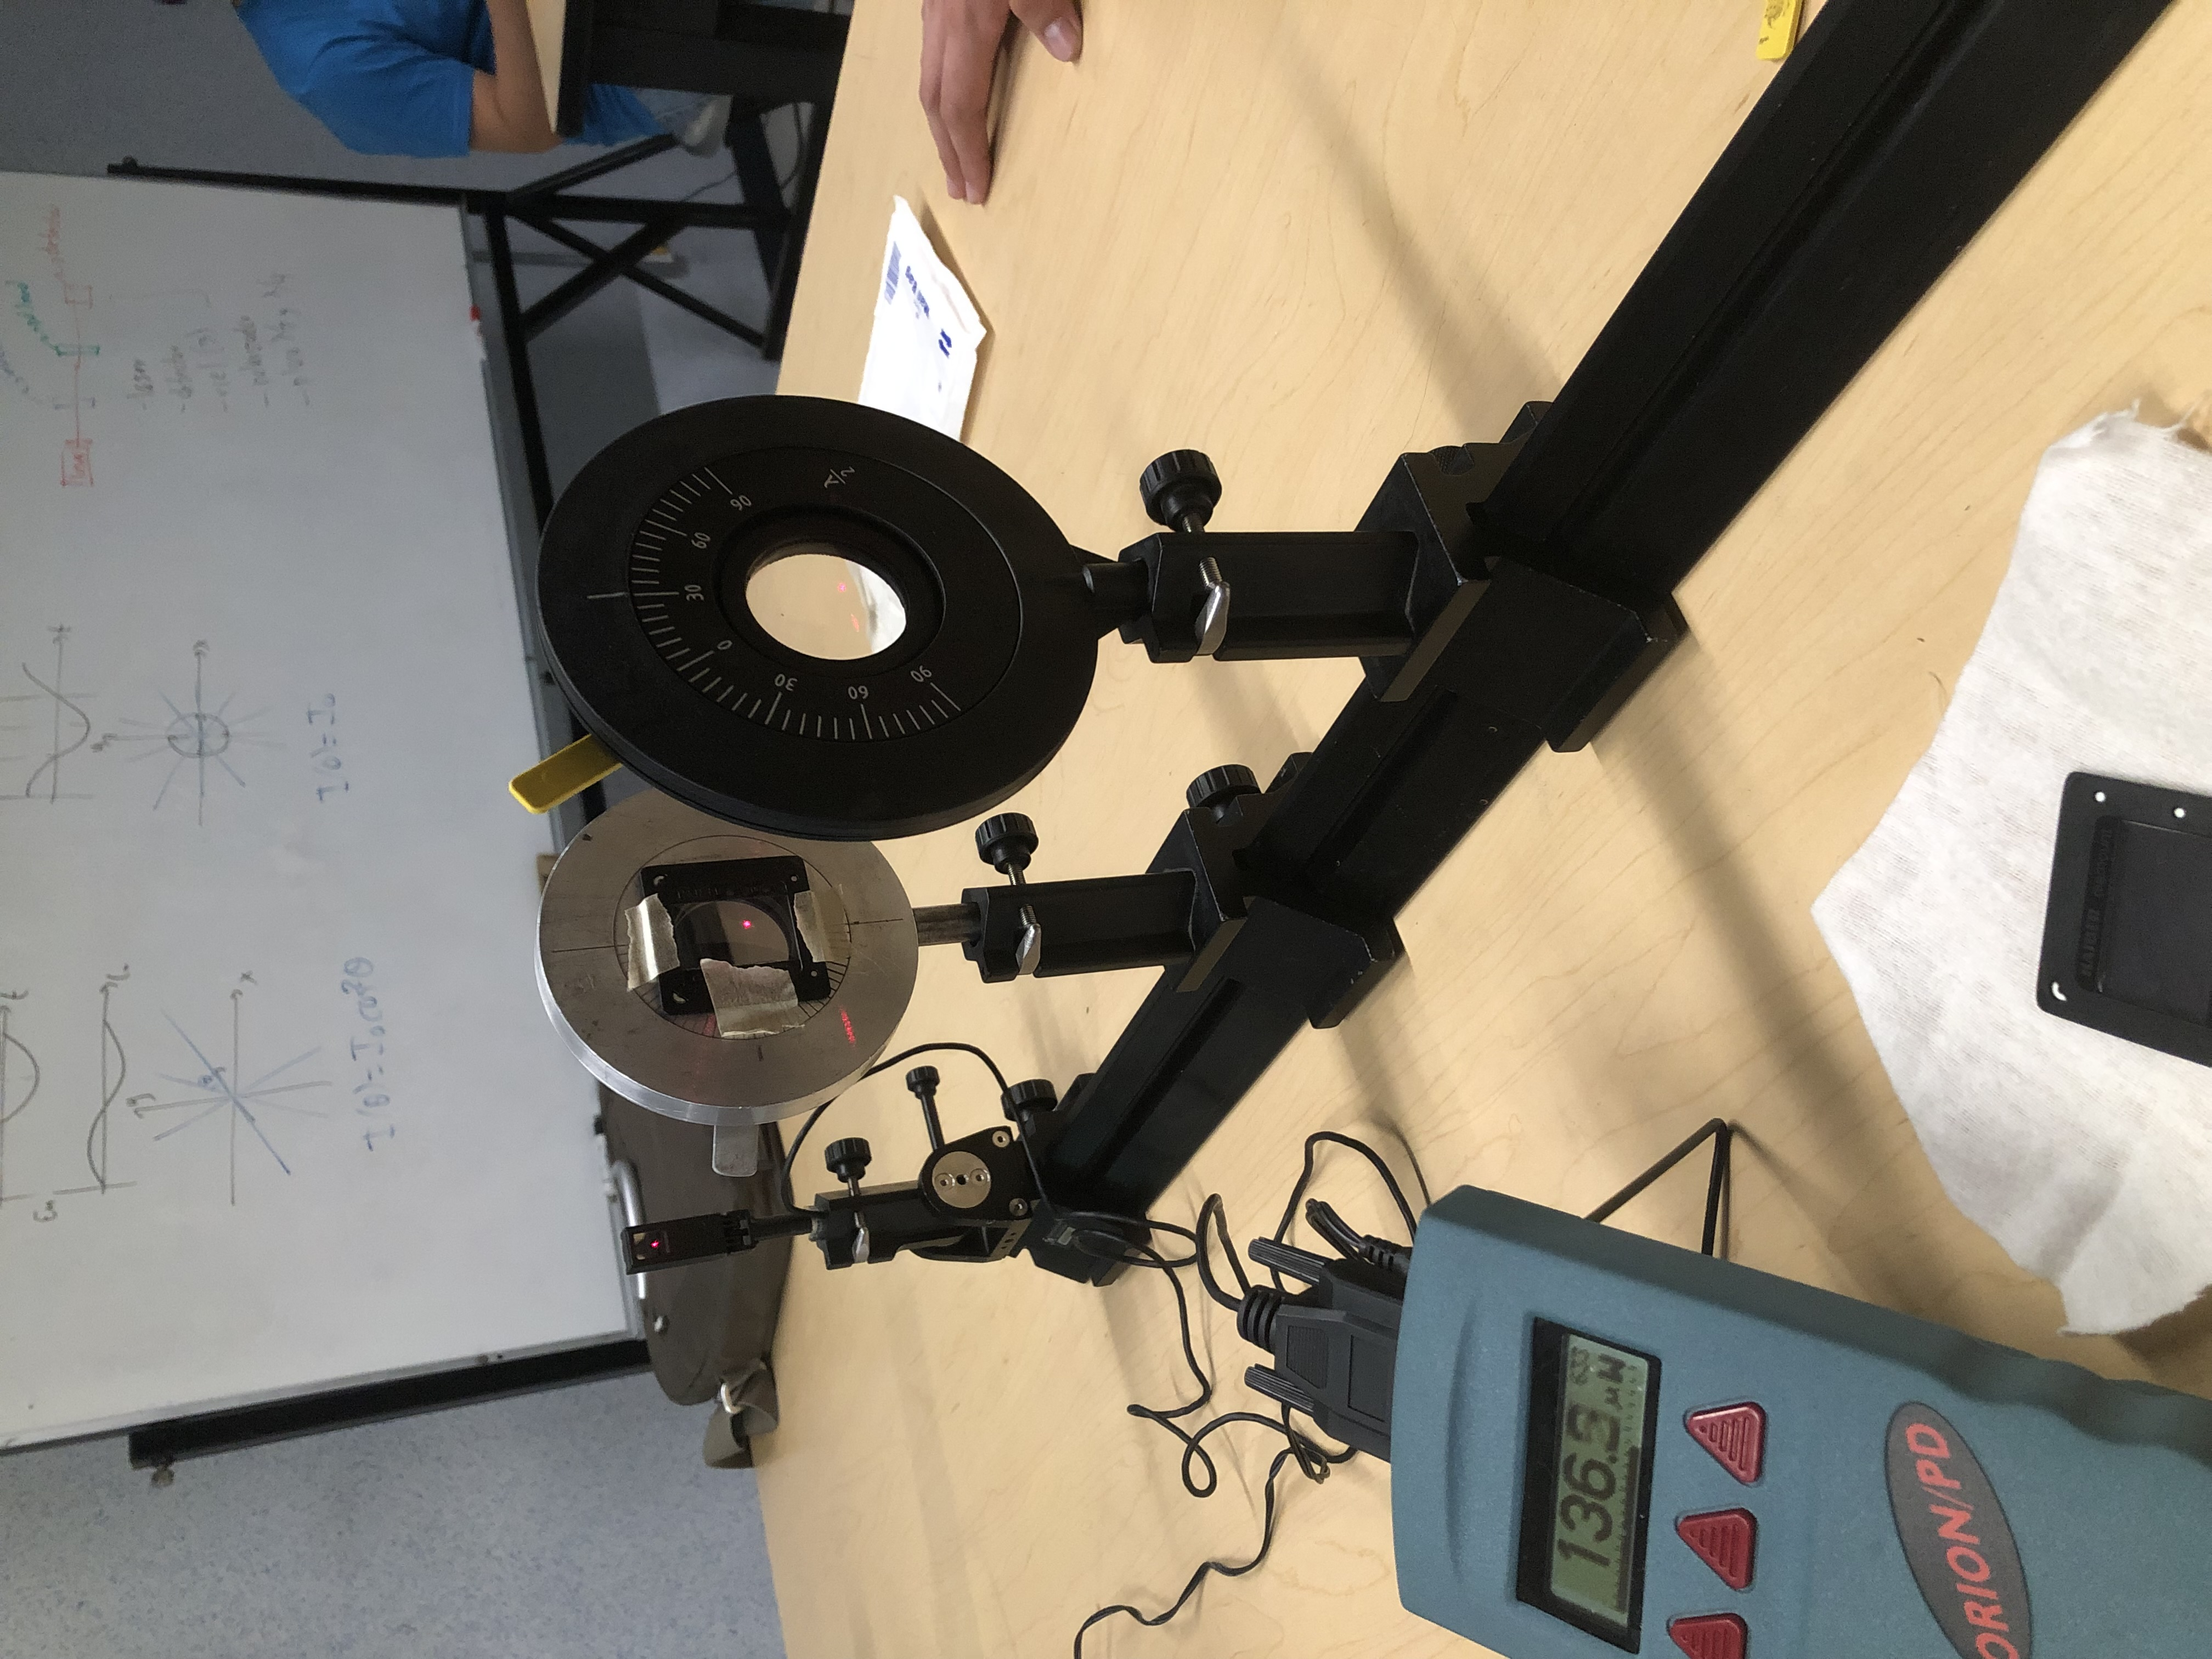
\includegraphics[width=0.9\linewidth, angle=-90]{Imagenes/labo.jpeg}
    \caption{Antes de incidir sobre el polarizador lineal (disco plateado), se introduce una diferencia de fases en el láser con un retardador de fase (disco negro).}
    \label{fig: labo}
\end{figure}

Posteriormente reemplazamos el retardador de $\lambda/2$ por uno de $\lambda/4$ con su eje rápido a \ang{45} y repetimos las 36 mediciones. Finalmente repetimos las mediciones con el retardador de un cuarto de longitud de onda a \ang{-50}.

\end{multicols}
%\begin{multicols}{2}
\end{multicols}

%\section{Conclusiones}



%\nocite{*}
\printbibliography

\end{document}
